% Printed 468; principal PDF 475; Google PDF 479.
\par\clearpage
\noindent\makebox[0pt][l]{\fontsize{13}{16}\selectfont 468}\hfill{\small\textbf{BRIEFWECHSEL.}}\hfill\null\par\medskip
\noindent erst nach ein paar Minuten eintreten würde. Wenn man sich dann mit dem Ablesen und Weiterrücken der Alhidade beeilt, gelingt es wohl, dass der Beobachter dort, wohin das Licht geworfen wird, über 2 Minuten den vollen Glanz genießt. Offenbar ist die Mühe unvergleichlich geringer, wenn direkt am großen Spiegel, senkrecht zur Ebene des Sextanten, unter der Neigung $a$ ein dritter Spiegel befestigt ist. Dadurch wird der Sextant zu einem vollständigen Sonnenspiegel. Er steht nur deshalb deutlich zurück, weil das kleine Fernrohr mit seinem halben Licht keine sehr großen Entfernungen überbrückt und weil dieser dritte Spiegel bei Bewegungen des Sextanten auf seinem Stativ nicht in Ruhe bleibt. Ich beabsichtige jedoch, für die Gegensignale einen solchen dritten Spiegel an meinem Sextanten anbringen zu lassen.

\par\noindent\hspace*{\parindent}Die bisherigen kleinen Versuche sind so verlaufen: \textls[120]{Zuerst}, nur auf der Terrasse der Sternwarte, bei einer Entfernung von 60 Metern, war das Licht so stark, dass man es nicht einmal einen Augenblick lang ohne Schmerzen ansehen konnte. \textls[120]{Zweitens}, etwas weiter unten, bei einer Entfernung von 150 Metern, war schon ein paar Sekunden langes Hinsehen schmerzhaft für das Auge. Nur diese beiden Versuche habe ich selbst gemacht, da ich bisher niemanden habe, der das Instrument einstellen könnte, und es also selbst tun musste. (Es wäre besser, jemand anderen dafür einzuarbeiten, wenn das Stativ nicht so unvollkommen ausbalanciert wäre, dass es äußerst behutsam behandelt werden muss, damit die Versuche nicht völlig misslingen. Sobald ein dritter Spiegel vorhanden ist, entfällt diese Schwierigkeit offensichtlich.) Bei den folgenden Versuchen haben teils der jetzt hier angestellte Professor \textsc{Ulrich}, teils Leutnant \textsc{Hartmann} beobachtet.

\par\noindent\hspace*{\parindent}Beim \textls[120]{dritten} Versuch betrug die Entfernung 300 Meter. Professor \textsc{Ulrich} beschrieb das Licht als herrlich und bei längerem Hinsehen für das Auge als anstrengend.

\par\noindent\hspace*{\parindent}Vorgestern \textls[120]{ein vierter Versuch}, auf eine Entfernung von 2000 Metern. Professor \textsc{Ulrich} bezeichnete das Licht wieder als herrlich und verglich es mit dem 3-fachen Glanz der Venus, wie sie nachts erscheint, wenn sie am schönsten ist. Sein Begleiter habe gar nicht genug zeigen können, wie sehr er darüber erstaunt sei, dass ein solcher Glanz hervorgebracht werden könne.

\par\noindent\hspace*{\parindent}Gestern \textls[120]{fünfter Versuch}, am Standort des künftig zu errichtenden \textls[120]{süd-}

% Printed 469; principal PDF 476; Google PDF 480.
\par\clearpage
\noindent\null\hfill{\small\textbf{HELIOTROP.}}\hfill\makebox[0pt][r]{\fontsize{13}{16}\selectfont 469}\par\medskip
\noindent\textls[120]{lichen} Meridianzeichens, wo ich eine Schneise durch einen beträchtlichen Wald schlagen lassen musste, bei einer Entfernung von 11890 Metern. Leutnant \textsc{Hartmann} nennt das Licht wieder \textls[120]{herrlich} und meint, dass es an Intensität wohl noch der Venus in der Abenddämmerung gleichgekommen, aber für das Auge, wie er sich ausdrückte, \textls[120]{beleidigender} gewesen sei. Selbstverständlich wurden alle diese Beobachtungen mit bloßem Auge gemacht. Ein Arbeiter, den er bei sich hatte, habe beim ersten Aufblitzen erschrocken Feuer gerufen. Im Fernrohr des Theodoliten schien der Faden an der Stelle dieses scharfen Lichtpunkts vollständig durchschnitten.

\par\noindent\hspace*{\parindent}Der Spiegel an meinem Sextanten ist genau 2 Pariser Zoll breit und $1\frac14$ Zoll hoch. Der Spiegel des von \textsc{Rumpf} angefertigten Heliotrops hat fast dieselben Abmessungen.

\par\noindent\hspace*{\parindent}Ich dachte, es würde Ihnen nicht unangenehm sein, diese Ergebnisse zu erfahren. Bis ich mit dem eigentlichen Sonnenspiegel noch einige Versuche in etwas größerem Maßstab durchgeführt habe, wäre mir lieber, wenn nichts davon nach außen dränge.

\par\noindent\hspace*{\parindent}Ich hoffe nun sehr, dass diese Vorrichtung auch bei den größten Entfernungen in meinem Dreieckssystem aushelfen wird. Ich glaube, wenn man die Sonnenspiegel nach der zweiten in meinem letzten Brief angedeuteten Anordnung ausführt und den Spiegel hinreichend groß macht, dann gelten künftig für die Länge der Dreiecksseiten nur noch die Grenzen, die die Kugelgestalt der Erde setzt.

\par\noindent\hspace*{\parindent}Vielleicht können diese Ideen auch in anderer Hinsicht noch wichtige Anwendungen finden, z. B. als Signale für astronomische Längenbestimmungen, da man das Licht jederzeit augenblicklich verdecken und wieder erscheinen lassen kann. Vielleicht eignen sie sich sogar für andere telegrafische Signale, wenigstens wenn die Sonne einigermaßen stetig scheint und den sehr genau zu messenden Zeitabständen zwischen Erscheinen und Verschwinden vereinbarte Bedeutungen zugeordnet werden.

\par\noindent\hspace*{\parindent}Mein Hohehagen-Signal ist gestern fertig geworden. Ich möchte noch diese Woche (wenn \textsc{Rumpf} Wort hält) die schwierige Justierung des Sonnenspiegels und die Messung des Winkels Hohehagen-Meridianzeichen hier abschließen und dann zum Hohehagen aufbrechen.\enspace .\ .\ .\ .\ .\ .

% Printed 470; principal PDF 477; Google PDF 481.
\par\clearpage
\noindent\makebox[0pt][l]{\fontsize{13}{16}\selectfont 470}\hfill{\small\textbf{BRIEFWECHSEL.}}\hfill\null\par\bigskip
\begin{center}{\large\textsc{Gauss} an \textsc{Schumacher}.\quad Göttingen, 11. Juli 1821.}\end{center}
\par\noindent\hspace*{\parindent}.\ .\ .\ .\ .\ .\enspace Vielleicht könnte eine Mitteilung über mein neues Instrument, dem ich den Namen Heliotrop geben möchte, den Anfang[\textsuperscript{*})] machen. Ich hoffe, dass diese Beobachtungsweise für die höhere Geodäsie von größter Bedeutung werden kann. Für kurze Entfernungen (bis 2 Meilen) können Sie sich keinen schöneren Zielpunkt vorstellen als das von einer hellen Wolke reflektierte Licht. Reflektiertes Sonnenlicht, so hoffe ich, wird auf die allergrößten Entfernungen das schönste Ziel bieten.\enspace .\ .\ .\ .\ .\ .
\par\bigskip
\begin{center}{\large\textsc{Gauss} an \textsc{Schumacher}.\quad Göttingen, 8. November 1821.}\end{center}
\par\noindent\hspace*{\parindent}.\ .\ .\ .\ .\ .\enspace Den Artikel über den Heliotrop in den Göttingischen gelehrten Anzeigen hat \textsc{Zach} in seiner Zeitschrift[\textsuperscript{**})] übersetzt. Die Übersetzung enthält jedoch mehrere Unrichtigkeiten. Von den beiden neuen Heliotropen ist einer jetzt fertig. Er hat eine prächtige Wirkung, nur fällt es uns sehr schwer, gute Spiegel zu bekommen. Die bisherigen sind äußerst schlecht, was zwar der Wirkung selbst wenig oder gar keinen Abbruch tut, aber die Justierung sehr erschwert. Gestern habe ich einen Versuch mit Mondlicht gemacht. In einer freilich nur kleinen Entfernung von etwa 250 Metern ergab sich eine überaus schöne Wirkung. Das Licht ähnelte dem der Venus (nachts, wenn sie hoch steht), war aber um ein Vielfaches brillanter. Das Telegrafieren habe ich ziemlich weit entwickelt. Nötigenfalls kann ich einige Tausend verschiedene Zeichen geben.\enspace .\ .\ .\ .\ .\ .
\par\bigskip
\begin{center}{\large\textsc{Gauss} an \textsc{Schumacher}.\quad Steinkrug am Deister, 10. Juli 1822.}\end{center}
\par\noindent\hspace*{\parindent}.\ .\ .\ .\ .\ .\enspace Ich habe dieses Jahr 3 eigentliche Heliotrope und noch einen weiteren Heliotropapparat im Einsatz. Zwei von jenen sind immer in der Ferne in Betrieb. Es ist eine Pracht (a luxury), in schönen Abendstunden Winkel zwischen zwei Heliotroplichtern zu messen, und die Übereinstimmung der Ergebnisse ist dann oft ganz erstaunlich.\enspace .\ .\ .\ .\ .\ .
\par\medskip\noindent\rule{4cm}{.4pt}\par
\begingroup\footnotesize
\noindent\hspace*{\parindent}[\textsuperscript{*}) \textsc{Schumacher} hatte um einen Beitrag für die Astronomischen Nachrichten gebeten.]\par
\noindent\hspace*{\parindent}[\textsuperscript{**}) Correspondance astronomique, géographique, etc. du Baron \textsc{de Zach}.\quad V. Band.\quad 1821, S. 374/382.]\par
\endgroup

% Printed 471; principal PDF 478; Google PDF 482.
\par\clearpage
\noindent\null\hfill{\small\textbf{HELIOTROP.}}\hfill\makebox[0pt][r]{\fontsize{13}{16}\selectfont 471}\par\bigskip
\begin{center}{\large\textsc{Gauss} an \textsc{Schumacher}.\quad Göttingen, 15. Januar 1827.}\end{center}
\par\noindent\hspace*{\parindent}Hiermit erhalten Sie den Aufsatz über die Justierung der Heliotrope zurück[\textsuperscript{*})]. Nur beim $3^{\mathrm{ten}}$ Verfahren zur $7^{\mathrm{ten}}$ Justierung hatte ich, wenn ich mich recht erinnere, eigentlich etwas anderes gemeint, als hier steht. Ich meinte, einen Sextanten so einzustellen, dass die Spiegel genau parallel sind, also den Index auf den \textls[120]{wahren} Nullpunkt zu stellen und, worauf es hier eigentlich ankommt, die Spiegel so zu justieren, dass sie senkrecht zur Ebene des Sextanten stehen. Hält man dann den Sextanten so, dass man das vom I. Spiegelbestandteil reflektierte Bild eines hellen, scharf begrenzten Gegenstands (Fixsterne erster Größe oder hinreichend entferntes Heliotroplicht wären besser als die Sonne) direkt sieht, das Bild vom II. Spiegelbestandteil dagegen durch die Reflexion an den beiden Spiegeln des Sextanten, also im Grunde durch dreimalige Reflexion, dann soll man nur ein Bild sehen. Ich muss jedoch zugeben, dass ich dieses Verfahren selbst nicht angewandt habe. Seine Brauchbarkeit hängt auch von den Abmessungen des Heliotrops und des Sextanten ab. Der Abstand zwischen den Mittelpunkten von I und II soll etwas kleiner sein als der Abstand des Mittelpunkts des großen Sextantenspiegels von der Achse des Fernrohrs. Sie können es also durchaus so stehen lassen, wie es
\begin{center}
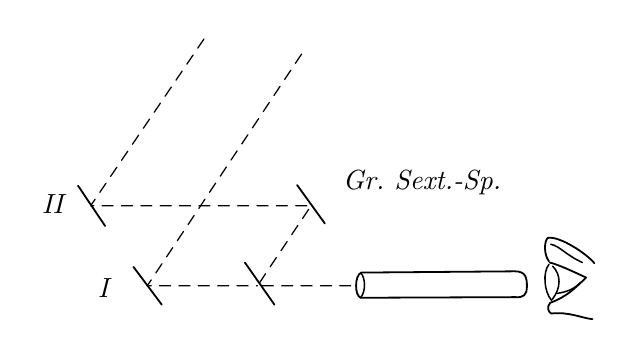
\begin{tikzpicture}[x=.008cm,y=-.008cm,line cap=round,line join=round]
\path[use as bounding box] (50,0) rectangle (970,475);
\draw[line width=.45pt,dash pattern=on 4pt off 3pt] (330,18)--(150,283)--(500,283)--(415,410)--(575,410);
\draw[line width=.45pt,dash pattern=on 4pt off 3pt] (485,42)--(240,410)--(415,410);
\draw[line width=.65pt] (130,251)--(173,315) (218,380)--(263,440) (478,250)--(522,311) (395,373)--(442,440);
\node[font=\itshape,anchor=east] at (122,280) {II};
\node[font=\itshape,anchor=east] at (194,414) {I};
\node[font=\itshape,anchor=west] at (535,247) {Gr.\ Sext.-Sp.};
\draw[line width=.65pt] (580,389)--(824,387)..controls (841,387) and (843,397)..(843,411)..controls (843,425) and (837,429)..(825,428)--(579,429)..controls (569,426) and (569,393)..(580,389);
\draw[line width=.55pt] (579,389)..controls (587,399) and (587,418)..(579,429);
\draw[line width=.65pt] (878,371)..controls (870,361) and (870,340)..(876,334)..controls (894,330) and (938,359)..(950,374);
\draw[line width=.55pt] (881,344)..controls (897,348) and (903,360)..(931,373);
\draw[line width=.65pt] (879,373)..controls (892,376) and (916,387)..(937,397)..controls (919,414) and (907,427)..(880,437)..controls (874,443) and (877,453)..(882,454)..controls (910,451) and (929,461)..(947,463);
\draw[line width=.55pt] (884,379)..controls (897,392) and (898,413)..(883,432);
\draw[line width=.55pt] (878,376)..controls (868,388) and (870,419)..(882,433);
\draw[line width=.55pt] (891,422)..controls (906,420) and (918,415)..(928,405);
\end{tikzpicture}
\end{center}
\noindent geschrieben ist, zumal jeder Leser die nötigen Vorsichtsmaßnahmen leicht selbst ergänzen kann. So stellt man das Spiegelsystem am besten so ein, dass die Sonne ungefähr in der Ebene liegt, auf der die Spiegelachse senkrecht steht. Wenn zwischen den Messungen an den beiden Spiegelbestandteilen etwas Zeit verstreicht (mehr als ein paar Sekunden, was ein geübter Beobachter wohl vermeiden kann), muss man das berücksichtigen.\enspace .\ .\ .\ .\ .\ .
\par\medskip\noindent\rule{4cm}{.4pt}\par
\begingroup\footnotesize\noindent\hspace*{\parindent}[\textsuperscript{*}) Siehe die folgende Abhandlung.]\par\endgroup
\begin{center}\rule{3.5cm}{.4pt}\end{center}

% Printed 472; principal PDF 479; Google PDF 483.
\par\clearpage
\noindent\makebox[0pt][l]{\fontsize{13}{16}\selectfont 472}\hfill{\small\textbf{HELIOTROP.}}\hfill\null\par
\vspace*{4.4cm}
\begin{center}
\begin{tabular}{c}\hline
\small\textbf{Astronomische Nachrichten, Bd. V, Nr. 116, Februar 1827, S. 329--334.}\\\hline
\end{tabular}\par\bigskip
{\large Die Justierung des Heliotrops.}
\end{center}
\par\noindent\hspace*{\parindent}Zur vollständigen Justierung des Heliotrops sind insgesamt acht Arbeitsschritte erforderlich:
\par\noindent\hangindent=1.8em\hangafter=1\hspace*{1em}1.\ 2.\quad Die optische Achse des Fernrohrs wird mit den Justierschrauben $E$ und $F$ (Fig. 1) parallel zu dessen Drehachse eingestellt.
\par\noindent\hangindent=1.8em\hangafter=1\hspace*{1em}3.\quad Die Spiegelachse $AB$ stellt man mit den Schrauben $CC$ (Fig. 1) am einen Arm der Gabel, die diese Achse trägt, senkrecht zur Drehachse des Fernrohrs ein.
\par\noindent\hangindent=1.8em\hangafter=1\hspace*{1em}4.\ 5.\ 6.\quad Die Ebenen der drei Spiegel (des kleineren und der beiden Bestandteile des größeren) werden mit den Schrauben $G$, $H$, $I$ (Fig. 2) parallel zur Spiegelachse eingestellt.
\par\noindent\hangindent=1.8em\hangafter=1\hspace*{1em}7.\quad Mit der Schraube $K$ (Fig. 2) wird der Bestandteil II des größeren Spiegels in eine zum Bestandteil I parallele Ebene gebracht.
\par\noindent\hangindent=1.8em\hangafter=1\hspace*{1em}8.\quad Der kleine Spiegel muss mit der Schraube an seinem hinteren Ende so eingestellt werden, dass die Ebene des Spiegels senkrecht auf den Ebenen der beiden Bestandteile des großen steht.
\par\noindent\hspace*{\parindent}Die Justierungen 1 und 2 übergehe ich als allgemein bekannt.

\par\noindent\hspace*{\parindent}Um die Justierung 3 ganz selbstständig auszuführen, stelle ich den Heliotrop auf einen festen Sockel, richte die Spiegelachse $AB$ (Fig. 3) vertikal mit dem Stiel $AD$ nach unten und drehe diesen Stiel, bis er zur Okularseite\textsuperscript{*}) hin parallel zur Fernrohrachse steht. Alles nur nach Augenmaß. An den Stiel $AD$ hänge ich eine nicht zu empfind-
\par\medskip\noindent\rule{4cm}{.4pt}\par
\begingroup\footnotesize\noindent\hspace*{\parindent}\textsuperscript{*}) Dies kann auch, mutatis mutandis, umgekehrt gemacht werden.\par\endgroup

% Printed 473; principal PDF 480; Google PDF 484.
\par\clearpage
\noindent\null\hfill{\small\textbf{HELIOTROP.}}\hfill\makebox[0pt][r]{\fontsize{13}{16}\selectfont 473}\par\medskip
\noindent liche Libelle und bringe die Blase durch Änderung der Länge der Drähte, an denen die Libelle aufgehängt ist, \textls[120]{annähernd} und danach mit den Fußschrauben \textls[120]{genau} zum Einspielen. Dann drehe ich den Stiel um $180^\circ$ um die Spiegelachse, hebe das Fernrohr vorsichtig aus und lege es in der entgegengesetzten Lage wieder ein (Fig. 4). Die Justierung ist unnötig, wenn die Blase dann wieder einspielt. Andernfalls wird die eine Hälfte des Ausschlags an den Fußschrauben und die andere an den Schrauben $CC$ (Fig. 1) korrigiert. Die Rückkehr in die vorige Lage zeigt, ob die Aufteilung richtig vorgenommen wurde. Die bei diesem Verfahren nötigen Vorsichtsmaßnahmen übergehe ich, da sie jeder auch ohne Anleitung finden wird und ich das Verfahren später entweder gar nicht oder nur für die erste grobe Justierung angewandt habe\textsuperscript{*}).

\par\noindent\hspace*{\parindent}Ein Verfahren, das ich für die Justierungen 4, 5 und 6 angewandt habe, beruht auf dem Prinzip, dass eine Ebene $ab$ (Fig. 5) durch eine halbe Umdrehung um eine zu ihr parallele Achse $AB$ in eine zu ihrer ersten Lage $ab$ parallele, aber entgegengesetzte Lage $cd$ gebracht wird. Sind die Achse und die Ebene dagegen nicht parallel, wie in Fig. 6, so werden auch die beiden Lagen $ab$ und $cd$ nicht parallel sein. Um dies an einem Spiegel zu prüfen, stelle ich zwei mit Kreuzfäden versehene Fernrohre $M$, $N$ (Fig. 7) so auf, dass deutlich erkennbare Objekte $O$, $P$ auf ihren optischen Achsen erscheinen und dass diese sich annähernd schneiden oder annähernd in einer Ebene liegen. Nachdem ich die Gabel vom Fernrohr abgenommen und auf einem Kästchen oder Brett befestigt habe, stelle ich den zu prüfenden Spiegel auf einem Tisch nahe dem Schnittpunkt der optischen Achsen auf, sodass die Drehachse $AB$ ungefähr in ihrer Ebene liegt und den Winkel zwischen ihnen halbiert. Dann stelle ich den Spiegel $L$ senkrecht zu jener Ebene und sorge durch kleine Drehungen und sanfte Stöße sowohl am Spiegel selbst als auch am Kästchen dafür, dass das vom Spiegel reflektierte Bild von $O$ auf der optischen Achse von $M$ erscheint. Darauf drehe ich den Spiegel um $180^\circ$ um seine Achse und prüfe, ob in dieser Lage (Fig. 8) das Bild von $P$ auf der optischen Achse von $N$ erscheint. Lässt sich dies durch bloßes Drehen des Spiegels um die Achse $AB$ nicht erreichen, so muss die eine Hälfte am Kästchen und die
\par\medskip\noindent\rule{4cm}{.4pt}\par
\begingroup\footnotesize\noindent\hspace*{\parindent}\textsuperscript{*}) Im Übrigen beruht die Brauchbarkeit dieser Methode darauf\rlap{\hspace{.05em}\raisebox{2ex}{.}}, dass die zylindrischen Ansätze, mit denen das Fernrohr in den Lagern ruht, genau gleich dick sind. Bei den von Herrn \textsc{Rumpf} angefertigten Instrumenten wurde dies sorgfältig berücksichtigt.\par\endgroup
\par\medskip\noindent\makebox[0pt][l]{\small IX.}\makebox[.86\linewidth][r]{60}\par

% Printed 474; principal PDF 481; Google PDF 485.
\par\clearpage
\noindent\makebox[0pt][l]{\fontsize{13}{16}\selectfont 474}\hfill{\small\textbf{HELIOTROP.}}\hfill\null\par\medskip
\noindent andere Hälfte an der Lage des Spiegels gegenüber seiner Achse korrigiert werden. Die Objekte $O$, $P$ brauchen nicht weit entfernt zu sein, sofern der Spiegel dicht an seiner Achse sitzt. Ich habe sie in einer Entfernung von etwa 70--80 Fuß aufgestellt.

\par\noindent\hspace*{\parindent}Für die Justierung 7 lassen sich verschiedene Verfahren anwenden. Das einfachste, das auch eine hinreichende Genauigkeit bietet, besteht darin, eine zur Spiegelachse ungefähr parallele Gerade in den beiden Hälften des großen Spiegels zu betrachten. Dort muss sie als eine Gerade erscheinen, was sich schon mit bloßem Auge sehr genau beurteilen lässt.\ \raisebox{.55ex}{.}\ Ich habe dazu die Fassade der Sternwarte benutzt. --- Ein zweites Verfahren besteht darin, ein feines Objekt (Heliotroplicht) mit einem Fernrohr mit großem Objektiv (Kometensucher) gleichzeitig in beiden Spiegeln zu betrachten und den Bestandteil II zu justieren, bis man nur ein Bild sieht. Offenbar erreicht man dadurch auch die Justierung 6, wenn 5 bereits vorgenommen wurde. --- Bei einem dritten Verfahren verwendet man die beiden Bestandteile des großen Spiegels als künstliche Horizonte und misst mit einem Sextanten die Sonnenhöhen. Sie müssen gleich sein, wenn die Justierung vorgenommen ist. --- Ein viertes Verfahren wird sich gleich ergeben.

\par\noindent\hspace*{\parindent}Für die $8^{\mathrm{te}}$ Justierung habe ich folgendes Verfahren am besten gefunden. Ich stelle den Heliotrop und ein Hilfsfernrohr mit Kreuzfäden so auf, dass die optische Achse des letzteren parallel zur Achse des Heliotropfernrohrs ist und in derselben Vertikalebene um etwa den halben Abstand der Mittelpunkte der beiden Bestandteile des großen Spiegels höher liegt (Fig. 9). Dazu richte ich den Heliotrop auf ein gut sichtbares entferntes Objekt, nehme das Fernrohr heraus und lege es in umgekehrter Lage wieder ein, nachdem das Hilfsfernrohr in der angegebenen Höhe auf dasselbe Objekt gerichtet worden ist. Die Spiegelachse wird darauf senkrecht gestellt, mit dem Bestandteil I nach oben. Durch Drehen des Spiegelsystems und nötigenfalls auch des Fernrohrs wird erreicht, dass ein Objekt durch Reflexion am kleinen Spiegel auf der optischen Achse des Heliotropfernrohrs erscheint. Erscheint dasselbe Objekt durch Reflexion am Bestandteil I des großen Spiegels auf der optischen Achse des Hilfsfernrohrs, so bildet die Ebene des kleinen Spiegels mit dem des Bestandteils I einen rechten Winkel. Andernfalls wird die Abweichung an der Schraube am hinteren Spiegelende korri-

% Printed 475; principal PDF 482; Google PDF 486.
\par\clearpage
\noindent\null\hfill{\small\textbf{HELIOTROP.}}\hfill\makebox[0pt][r]{\fontsize{13}{16}\selectfont 475}\par\medskip
\noindent giert. Die Justierung 7 kann dann auch auf dieselbe Weise geprüft werden, indem man das Heliotropfernrohr um $180^\circ$ um seine Achse dreht, sodass der Bestandteil II oben liegt. Dabei müssen offensichtlich Objekte auf der anderen Seite gewählt werden.

\par\noindent\hspace*{\parindent}Die bisher beschriebenen Verfahren sind alle voneinander unabhängig. Die einzige Einschränkung ist, dass 7 nach 6 vorgenommen werden muss, weil eine Berührung der Schraube $I$ die Justierung 7 beeinflussen würde. Für die Justierung 3, sofern 4 bereits vorgenommen worden ist, oder für beide zugleich habe ich jedoch ein Verfahren angewandt, das auf dem Prinzip beruht, dass eine Fläche, die um eine zu ihr senkrechte Achse gedreht wird, stets in derselben Ebene bleibt. Wird also der kleine Spiegel senkrecht zur Achse des Heliotropfernrohrs gestellt (was auf zwei Arten geschehen kann, indem nämlich die reflektierende Fläche dem Fernrohr \textls[120]{zu-} oder von ihm \textls[120]{abgewandt} wird), so muss das Bild jedes Objekts in diesem Spiegel in Ruhe bleiben, während man das Fernrohr um seine Achse dreht. Ich stelle deshalb den kleinen Spiegel zunächst nach Augenmaß senkrecht zur Fernrohrachse, mit der reflektierenden Fläche vom Objektiv abgewandt (Fig. 10). Zur genaueren Einstellung beurteile ich zunächst mit bloßem Auge, ob das Bild eines seitlich liegenden Gegenstands bei Drehung des Fernrohrs um seine Achse unbeweglich bleibt. Bei senkrechter Spiegelachse stelle ich dann ein Hilfsfernrohr mit Kreuzfäden so auf, dass das vom kleinen Spiegel reflektierte Bild eines seitlich liegenden Gegenstands auf der optischen Achse des Hilfsfernrohrs erscheint, und zwar so, dass diese Achse annähernd auf die Mitte des kleinen Spiegels gerichtet ist. Ich drehe jetzt das Heliotropfernrohr eine halbe Umdrehung um seine Achse und prüfe, ob das reflektierte Bild auf der optischen Achse des Hilfsfernrohrs geblieben ist. Andernfalls wird die Hälfte der Abweichung nach links oder rechts durch Drehen des Spiegelsystems, die Hälfte der Abweichung nach oben oder unten aber an den Schrauben $CC$ (Fig. 1) korrigiert. Das Hilfsfernrohr\textsuperscript{*}) wird wieder so gerichtet, dass das reflektierte Bild genau auf der optischen Achse erscheint. Eine weitere halbe Umdrehung des Heliotropfernrohrs um seine Achse zeigt dann, ob die Aufteilung richtig vorgenommen wurde. Die Ebene des kleinen Spiegels $ab$ (Fig. 11) steht also jetzt genau senkrecht zur Fernrohrachse,
\par\medskip\noindent\rule{4cm}{.4pt}\par
\begingroup\footnotesize\noindent\hspace*{\parindent}\textsuperscript{*}) Oder der Heliotrop, was sich aber ohne Gehilfen nicht leicht machen lässt.\par\endgroup
\par\medskip\noindent\makebox[.86\linewidth][r]{60\textsuperscript{*}}\par

% Printed 476; principal PDF 483; Google PDF 487.
\par\clearpage
\noindent\makebox[0pt][l]{\fontsize{13}{16}\selectfont 476}\hfill{\small\textbf{HELIOTROP.}}\hfill\null\par\medskip
\noindent sodass, wenn die Justierung 4 bereits vorgenommen ist, auch 3 genau ausgeführt ist. Ist aber die Ebene des kleinen Spiegels nicht parallel zur Achse $AB$ (Fig. 11), so lässt sich der Spiegel durch Drehen des Spiegelsystems nicht in eine entgegengesetzte, zur Fernrohrachse senkrechte Lage bringen. Vielmehr weicht er bei der größten Abweichung um das Doppelte seiner Neigung gegen die Spiegelachse von ihr ab (Fig. 12). Man wiederhole also den vorigen Versuch in dieser Lage, wobei das Objekt in einer Richtung liegen muss, die mit der Fernrohrachse einen stumpfen Winkel bildet (Fig. 13). Ist der Spiegel nun so eingestellt, dass das reflektierte Bild, das zuerst bei senkrechter Spiegelachse auf der optischen Achse erschien, nach einer halben Umdrehung um die Fernrohrachse weder rechts noch links erscheint, so sind, sofern es auch weder höher noch tiefer liegt, die Justierungen 3 und 4 beide genau ausgeführt. Andernfalls wird von der Abweichung $\frac14$ an der Schraube $CC$ (Fig. 1) und $\frac14$ an der Schraube $G$ korrigiert. Das Hilfsfernrohr wird dann wieder auf das reflektierte Bild gerichtet. Nach einer halben Umdrehung des Heliotropfernrohrs um seine Achse prüft man, ob das Bild auf der optischen Achse geblieben ist. Wenn noch etwas nachzustellen ist, empfiehlt es sich, die Prüfung in der ersten Lage des Spiegels zu wiederholen. Die Objekte brauchen dazu nicht weit entfernt zu sein, sofern das Fadensystem des Hilfsfernrohrs auf diese Entfernung eingestellt ist.
\par\vspace{2.5cm}\begin{center}\rule{3.5cm}{.4pt}\end{center}

% Printed 477; principal PDF 484; Google PDF 488.
\par\clearpage
\noindent\null\hfill{\small\textbf{HELIOTROP.}}\hfill\makebox[0pt][r]{\fontsize{13}{16}\selectfont 477}\par\bigskip
\begin{center}
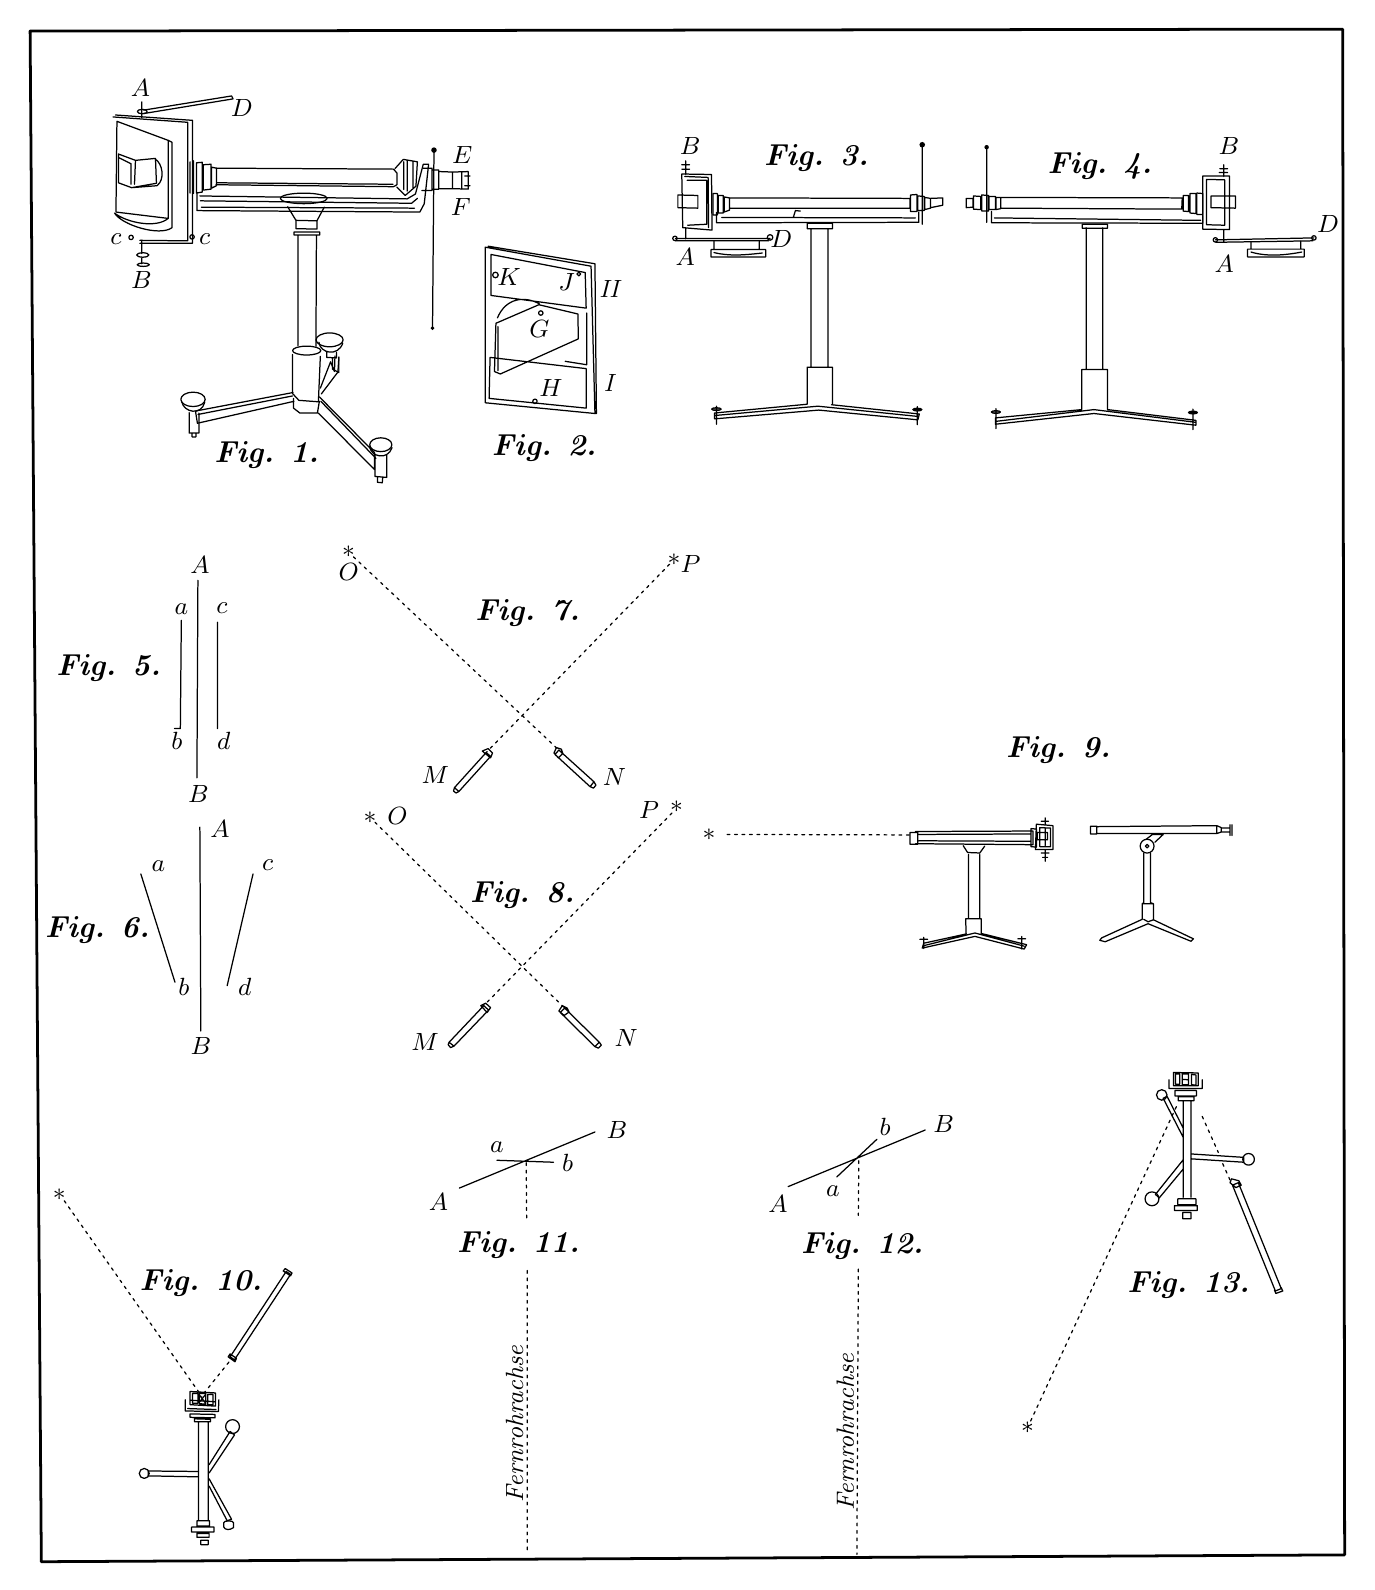
\begin{tikzpicture}[x=.0062cm,y=-.0062cm,line cap=round,line join=round,line width=.45pt,
  every node/.style={font=\fontsize{9}{10}\selectfont\itshape,inner sep=0pt},
  ray/.style={line width=.45pt,dash pattern=on 1pt off 1.7pt},
  caption/.style={font=\fontsize{11}{12}\selectfont\bfseries\itshape}]
\path[use as bounding box] (30,415) rectangle (2735,3560);
\draw[line width=1pt] (35,422)--(2726,418)--(2730,3546)--(58,3560)--cycle;
% Figures 1 and 2: perspective instrument and its mirror system.
\begin{scope}[shift={(110,500)}]
\draw (95,98)--(248,109)--(248,352)--(150,351)
 (100,94)--(258,105)--(258,357)--(150,357)
 (103,107)--(208,146)--(208,306)--(101,293)--cycle;
\draw (98,295)..controls (112,319) and (190,344)..(216,325)--(216,150)--(208,146)
 (98,295)..controls (123,315) and (184,327)..(208,306);
\draw (106,174)--(141,187)--(182,183)--(184,234)--(133,243)--(106,233)--cycle
 (141,187)--(139,236) (106,181)--(132,194)--(132,236)
 (181,184)..controls (197,193) and (202,227)..(185,239)--(133,243);
\draw (154,67)--(154,100) (158,84)--(338,55)--(341,61)--(158,91)
 (154,351)--(154,378) (154,387)--(154,399);
\draw (155,87) ellipse[x radius=1.8pt,y radius=.8pt]
 (156,381) ellipse[x radius=2.2pt,y radius=.8pt]
 (157,401) ellipse[x radius=2.2pt,y radius=.6pt];
\draw (132,345) circle[radius=.8pt] (257,344) circle[radius=.8pt];
\node at (151,39) {$A$}; \node at (359,80) {$D$}; \node at (153,432) {$B$};
\node at (101,348) {$c$}; \node at (283,349) {$c$};
\draw (253,190)--(253,254) (260,188)--(260,255)
 (266,192)--(278,191)--(278,252)--(266,254)--cycle
 (280,196)--(296,195)--(296,246)--(280,248)--cycle
 (297,201)--(307,203)--(307,239)--(297,244)--cycle;
\draw (307,203)--(670,205)--(677,213)--(677,237)--(670,241)--(306,237)
 (308,233)--(669,236)
 (673,204)--(690,185)--(719,190)--(716,240)--(694,259)--(677,242)
 (691,190)--(691,247) (698,188)--(698,250) (710,190)--(710,243);
\draw (273,260)--(698,266)--(715,256)--(731,195)--(742,195)--(733,276)--(724,293)--(267,290)--(267,254)
 (274,270)--(707,275)--(719,265) (276,283)--(713,285)
 (731,203)--(749,203)--(749,249)--(728,249)
 (750,207)--(763,207)--(763,246)--(750,246)
 (765,210)--(791,211)--(791,245)--(765,245)
 (791,211)--(823,210)--(823,246)--(791,245)
 (810,211)--(810,246) (816,219)--(827,219) (816,239)--(827,239);
\draw (753,167)--(750,531);
\fill (753,166) circle[radius=1pt] (750,531) circle[radius=.7pt];
\node at (811,177) {$E$}; \node at (808,282) {$F$};
\draw (486,265) ellipse[x radius=8.5pt,y radius=1.9pt];
\draw (453,282)--(470,310)--(513,311)--(528,283)
 (470,310)--(470,327)--(513,328)--(513,311)
 (466,334)--(519,334)--(519,340)--(466,340)--cycle
 (474,341)--(474,567) (512,342)--(511,568)
 (463,585)--(463,665)--(476,679)--(516,682)--(520,589);
\draw (492,577) ellipse[x radius=5.1pt,y radius=1.6pt];
\draw (465,675)--(465,695)--(478,705)--(514,705)--(518,681)
 (464,663)--(264,701)--(268,726)--(466,681)
 (269,708)--(463,670)
 (518,672)--(631,786)--(631,821)--(516,705)
 (521,681)--(634,798)
 (520,654)--(541,600)--(549,620)--(550,588)
 (522,666)--(556,621)--(558,591);
\draw (259,677) ellipse[x radius=4.4pt,y radius=2.6pt]
 (539,555) ellipse[x radius=4.9pt,y radius=2.5pt]
 (644,770) ellipse[x radius=4pt,y radius=2.5pt];
\draw (236,682)..controls (240,704) and (276,711)..(283,683)
 (251,704)--(251,746)--(271,746)--(271,705)
 (257,746)--(257,754)--(265,754)--(265,747)
 (517,560)..controls (520,583) and (556,590)..(566,562)
 (533,580)--(533,591)--(553,592)--(553,581)
 (545,592)--(545,615)--(558,622)--(558,590)
 (621,773)..controls (623,795) and (658,803)..(667,776)
 (632,790)--(632,835)--(656,837)--(656,791)
 (637,836)--(637,847)--(647,848)--(648,836);
\node[caption] at (410,790) {Fig. 1.};
\draw (858,365)--(1075,404)--(1083,706)--(858,684)--cycle
 (864,363)--(1083,399)--(1086,706)--(1083,706)
 (870,380)--(1063,417)--(1065,490)--(870,464)--cycle
 (868,591)--(1065,614)--(1065,695)--(866,675)--cycle
 (880,521)--(968,483)--(1048,502)--(1049,553)--(889,625)--(877,620)--cycle
 (884,528)--(884,618)
 (883,510)..controls (901,468) and (939,465)..(969,481)
 (1066,500)--(1066,606)--(1022,599);
\draw (879,422) circle[radius=1pt] (1050,420) circle[radius=.7pt]
 (972,500) circle[radius=.8pt] (960,681) circle[radius=.8pt];
\node at (907,427) {$K$}; \node at (1025,437) {$J$};
\node at (969,533) {$G$}; \node at (993,653) {$H$};
\node at (1112,450) {II}; \node at (1111,644) {I};
\node[caption] at (979,776) {Fig. 2.};
\end{scope}
% Figures 3 and 4: the two separately drawn positions with hanging level.
\begin{scope}[shift={(1310,600)}]
\draw (61,115)--(122,116)--(123,230)--(63,225)--cycle
 (67,120)--(115,122)--(116,225) (72,128)--(112,128)--(112,218)--(73,220)
 (53,158)--(94,159)--(94,185)--(53,184)--cycle
 (69,88)--(69,116) (61,96)--(77,96) (61,105)--(77,105)
 (69,225)--(69,248) (48,247)--(242,247) (48,252)--(239,252);
\draw (47,247) circle[radius=.8pt] (242,245) circle[radius=1pt];
\draw (127,252)--(127,270) (220,253)--(220,269)
 (121,270)--(233,270)--(233,285)--(121,285)--cycle
 (127,276)..controls (159,284) and (190,281)..(226,277);
\node at (68,285) {$A$}; \node at (78,57) {$B$}; \node at (265,248) {$D$};
\draw (125,155)--(134,155)--(134,199)--(125,199)--cycle
 (136,159)--(146,159)--(146,195)--(136,195)--cycle
 (148,162)--(159,164)--(159,189)--(148,193)--cycle
 (159,164)--(529,165)--(529,185)--(159,185)
 (132,194)--(132,215)--(547,214)--(547,193)
 (143,204)--(540,205) (290,203)--(294,190)--(304,191)
 (530,158)--(543,157)--(543,192)--(530,192)--cycle
 (545,160)--(558,161)--(558,190)--(545,190)--cycle
 (559,163)--(571,165)--(571,185)--(559,188)--cycle
 (571,165)--(596,164)--(596,179)--(571,184)
 (554,55)--(554,218);
\fill (554,55) circle[radius=1pt];
\draw (318,216)--(370,216)--(370,227)--(318,227)--cycle
 (326,227)--(326,510) (361,227)--(361,510)
 (318,511)--(370,511)--(370,588)
 (318,511)--(318,587)--(128,605)--(128,617)--(342,599)--(545,619)--(548,607)--(368,588)
 (130,610)--(340,591)--(545,612)
 (132,591)--(132,628) (123,597)--(141,597)
 (544,592)--(544,629) (535,598)--(553,598);
\draw (132,597) ellipse[x radius=1.7pt,y radius=.5pt]
 (544,598) ellipse[x radius=1.6pt,y radius=.5pt];
\node[caption] at (337,83) {Fig. 3.};
\draw (644,165)--(658,165)--(658,183)--(644,184)--cycle
 (659,160)--(674,161)--(674,188)--(659,187)--cycle
 (676,158)--(690,159)--(690,191)--(676,191)--cycle
 (691,161)--(704,161)--(704,188)--(691,188)--cycle
 (705,163)--(715,163)--(715,186)--(705,188)--cycle
 (715,163)--(1087,164)--(1086,187)--(715,185)
 (1089,159)--(1100,159)--(1100,192)--(1089,191)--cycle
 (1103,155)--(1115,155)--(1115,196)--(1103,195)--cycle
 (1117,154)--(1129,155)--(1129,198)--(1117,198)--cycle
 (702,205)--(1125,210) (696,192)--(696,215)--(1129,216)--(1129,200)
 (686,60)--(686,214);
\fill (686,60) circle[radius=.8pt];
\draw (1129,119)--(1184,119)--(1184,229)--(1129,228)--cycle
 (1137,126)--(1174,127)--(1174,220)--(1137,219)--cycle
 (1146,160)--(1196,160)--(1196,185)--(1146,184)--cycle
 (1172,96)--(1172,120) (1164,104)--(1180,104) (1163,112)--(1180,112)
 (1172,230)--(1172,253) (1155,250)--(1357,246) (1156,255)--(1355,252);
\draw (1155,250) circle[radius=.8pt] (1357,246) circle[radius=.8pt];
\draw (1228,254)--(1228,269) (1330,253)--(1330,269)
 (1221,269)--(1337,269)--(1337,285)--(1221,285)--cycle
 (1228,275)..controls (1265,286) and (1305,280)..(1332,275);
\node at (1173,300) {$A$}; \node at (1183,57) {$B$}; \node at (1386,217) {$D$};
\draw (882,218)--(934,218)--(934,226)--(882,226)--cycle
 (890,225)--(890,515) (924,225)--(924,515)
 (881,516)--(934,516)--(934,598)
 (881,516)--(881,598)--(704,615)--(704,628)--(906,606)--(1115,630)--(1115,620)--(934,598)
 (706,622)--(906,598)--(1114,624)
 (705,596)--(705,637) (696,603)--(714,603)
 (1109,597)--(1109,639) (1100,604)--(1118,604);
\draw (705,603) ellipse[x radius=1.6pt,y radius=.5pt]
 (1109,604) ellipse[x radius=1.6pt,y radius=.5pt];
\node[caption] at (918,98) {Fig. 4.};
\end{scope}
% Figures 5 and 6: finite, unequal line segments without arrows.
\begin{scope}[shift={(70,1470)}]
\draw (309,78)--(307,483) (275,160)--(273,382)--(261,382) (349,164)--(349,382);
\node at (313,47) {$A$}; \node at (310,516) {$B$};
\node at (275,137) {$a$}; \node at (266,408) {$b$};
\node at (358,135) {$c$}; \node at (362,408) {$d$};
\node[caption] at (126,257) {Fig. 5.};
\draw (313,584)--(315,1002) (192,680)--(262,902) (422,680)--(369,909);
\node at (354,587) {$A$}; \node at (315,1033) {$B$};
\node at (228,663) {$a$}; \node at (280,912) {$b$};
\node at (452,661) {$c$}; \node at (405,912) {$d$};
\node[caption] at (103,795) {Fig. 6.};
\end{scope}
% Figures 7 and 8: crossing rays and two separate telescopes in each figure.
\begin{scope}[shift={(650,1450)}]
\node at (38,40) {$\ast$}; \node at (705,55) {$\ast$};
\node at (38,80) {$O$}; \node at (739,64) {$P$};
\draw[ray] (48,50)--(469,446) (696,65)--(320,451);
\draw (255,523)--(320,451)--(329,459)--(264,531)--cycle
 (312,448)--(324,443)--(333,452)--(329,462)--cycle
 (255,523)--(253,530)--(258,534)--(264,531)
 (469,446)--(541,511)--(533,521)--(461,455)--cycle
 (464,441)--(474,444)--(477,453)--(468,462)--(459,452)--cycle
 (541,511)--(545,518)--(540,524)--(533,521);
\node at (216,497) {$M$}; \node at (583,501) {$N$};
\node[caption] at (405,165) {Fig. 7.};
\node at (82,584) {$\ast$}; \node at (710,563) {$\ast$};
\node at (138,582) {$O$}; \node at (654,568) {$P$};
\draw[ray] (92,594)--(481,975) (701,575)--(315,970);
\draw (244,1045)--(315,970)--(325,979)--(254,1053)--cycle
 (309,970)--(319,965)--(329,974)--(322,984)--cycle
 (244,1045)--(242,1050)--(247,1056)--(254,1053)
 (481,975)--(552,1045)--(543,1054)--(472,984)--cycle
 (476,970)--(486,975)--(490,983)--(480,990)--(469,981)--cycle
 (552,1045)--(556,1051)--(550,1057)--(543,1054);
\node at (195,1044) {$M$}; \node at (607,1036) {$N$};
\node[caption] at (394,743) {Fig. 8.};
\end{scope}
% Figure 9: heliotrop and auxiliary telescope, separately elevated.
\begin{scope}[shift={(1380,1820)}]
\node at (47,250) {$\ast$}; \draw[ray] (84,249)--(459,250);
\draw (459,245)--(475,245)--(475,269)--(459,269)--cycle
 (470,243)--(711,242)--(711,270)--(470,268)
 (477,249)--(705,248) (477,262)--(705,263)
 (707,237)--(718,238)--(718,275)--(707,274)--cycle
 (718,228)--(752,231)--(752,280)--(716,280)--cycle
 (725,235)--(747,236)--(747,274)--(725,274)--cycle
 (736,237)--(736,272) (720,245)--(741,245)--(741,260)--(720,260)--cycle
 (736,215)--(736,229) (728,222)--(743,222)
 (736,280)--(736,304) (728,287)--(744,287) (731,296)--(741,296);
\draw (568,272)--(577,286)--(602,287)--(612,273)
 (579,290)--(579,422) (602,290)--(602,422)
 (573,422)--(605,422)--(605,452)--(698,475)--(693,484)--(592,458)--(484,482)--(487,472)--(574,453)--cycle
 (487,477)--(592,451)--(693,478)
 (487,460)--(487,483) (479,464)--(495,464)
 (688,458)--(688,484) (680,463)--(696,463);
\draw (829,232)--(842,232)--(842,248)--(829,248)--cycle
 (841,233)--(1088,231)--(1088,247)--(841,247)
 (1088,231)--(1097,235)--(1097,244)--(1088,247)
 (1097,236)--(1115,236)--(1115,244)--(1097,244)
 (1115,229)--(1115,251) (1119,229)--(1119,251)
 (961,265)--(978,249)--(956,249)--(943,259);
\draw (945,273) circle[radius=2.5pt] (945,273) circle[radius=.65pt];
\draw (938,287)--(938,389)--(935,391)--(935,423)--(852,461)--(848,466)--(859,469)--(947,432)--(1035,468)--(1040,463)--(958,424)--(958,391)--(952,389)--(952,287)
 (935,391)--(958,391) (938,423)--(947,428)--(958,424);
\node[caption] at (763,76) {Fig. 9.};
\end{scope}
% Figure 10: end-on instrument, oblique auxiliary telescope and ray.
\begin{scope}[shift={(55,2710)}]
\node at (40,98) {$\ast$};
\draw[ray] (50,110)--(332,511) (336,505)--(393,434);
\draw (390,430)--(505,255)--(514,261)--(399,436)--cycle
 (499,254)--(503,249)--(517,258)--(514,264)--cycle
 (386,430)--(390,424)--(403,433)--(400,440)--cycle;
\draw (308,501)--(360,504)--(360,531)--(308,528)--cycle
 (313,505)--(324,505)--(324,525)--(313,525)--cycle
 (327,505)--(340,505)--(340,527)--(327,526)--cycle
 (344,507)--(355,507)--(355,528)--(344,528)--cycle
 (327,508)--(339,524) (339,508)--(327,523)
 (309,519)--(360,522)
 (298,518)--(298,541)--(366,542)--(367,518)
 (303,536)--(361,538) (308,547)--(359,548)--(359,555)--(308,554)--cycle
 (317,557)--(350,558)--(350,563)--(317,563)--cycle
 (325,563)--(325,765) (345,563)--(345,764);
\draw (325,665)--(222,664)--(222,674)--(325,676)
 (347,651)--(390,583)--(399,590)--(347,668)
 (347,695)--(384,766)--(393,763)--(347,680);
\draw (214,669) circle[radius=1.8pt] (395,573) circle[radius=2.5pt];
\draw (377,770)..controls (377,765) and (397,765)..(397,770)--(397,780)..controls (389,786) and (380,785)..(377,779)--cycle
 (322,766)--(348,766)--(348,777)--(322,777)--cycle
 (311,779)--(357,779)--(357,789)--(311,789)--cycle
 (322,792)--(347,792)--(347,800)--(322,800)--cycle
 (330,806)--(345,806)--(345,815)--(330,815)--cycle;
\node[caption] at (330,278) {Fig. 10.};
\end{scope}
% Figures 11 and 12: the unlike inclinations are retained.
\begin{scope}[shift={(790,2630)}]
\draw (125,164)--(403,49) (202,107)--(318,111);
\node at (82,192) {$A$}; \node at (448,44) {$B$};
\node at (202,80) {$a$}; \node at (347,112) {$b$};
\draw[ray] (262,112)--(263,229) (264,333)--(264,915);
\node[caption] at (246,280) {Fig. 11.};
\node[rotate=90] at (238,647) {Fernrohrachse};
\draw (799,161)--(1080,45) (899,141)--(981,64);
\node at (778,196) {$A$}; \node at (1118,33) {$B$};
\node at (891,170) {$a$}; \node at (998,38) {$b$};
\draw[ray] (944,108)--(943,220) (943,330)--(940,915);
\node[caption] at (951,282) {Fig. 12.};
\node[rotate=90] at (916,664) {Fernrohrachse};
\end{scope}
% Figure 13: reverse position, its own oblique ray and auxiliary telescope.
\begin{scope}[shift={(2000,2490)}]
\draw[ray] (385,137)--(80,795) (438,157)--(471,231) (480,254)--(497,292);
\node at (80,796) {$\ast$};
\draw (370,82)--(370,100)--(438,100)--(438,82)
 (379,67)--(430,68)--(430,94)--(379,94)--cycle
 (383,70)--(392,70)--(392,91)--(383,91)--cycle
 (397,70)--(410,70)--(410,92)--(397,92)--cycle
 (397,81)--(410,82)
 (416,71)--(425,72)--(425,93)--(416,92)--cycle
 (382,104)--(426,104)--(426,115)--(382,115)--cycle
 (389,117)--(421,117)--(421,125)--(389,125)--cycle
 (399,125)--(399,323) (415,125)--(415,323)
 (399,200)--(358,120)--(366,116)--(399,181)
 (415,234)--(523,241)--(523,251)--(415,244)
 (399,246)--(342,317)--(350,324)--(399,265);
\draw (355,113) circle[radius=1.9pt] (533,245) circle[radius=2.1pt]
 (335,326) circle[radius=2.5pt];
\draw (388,326)--(425,326)--(425,338)--(388,338)--cycle
 (381,340)--(428,340)--(428,350)--(381,350)--cycle
 (398,354)--(415,354)--(415,367)--(398,367)--cycle
 (500,298)--(588,515)--(600,510)--(512,293)--cycle
 (495,293)--(498,285)--(513,289)--(518,298)--(507,303)--cycle
 (586,513)--(589,520)--(603,515)--(600,508);
\node[caption] at (410,502) {Fig. 13.};
\end{scope}
\end{tikzpicture}
\end{center}
